\cotefile{157-3}
\scanpage{222}
\mspage{172}
% L1–9
\uline{NB} Le groupe $\pi_1(X,x)$ est défini via la théorie du groupoïde fondamental. On sait qu'il est en bijection canonique avec $\pi_0(\Omega^1(X,x))$, où $\Omega^{\deleted{\unsure{1}}}(X,x)=\underline{\mathrm{Ch}}(X;x,x)$ (ce qui permet d'avoir une loi de composition monoïdale sur $\Omega^1(X,x)$, donnant la loi de groupe sur le $\pi_0$), ou au choix $\Omega^{\deleted{\unsure{1}}}(X,x)=\mathrm{Ch}_{\infty}(X;x,x)$ (plus commode dans certaines situations, mais ne donnant pas \inserted{directement} la loi de composition du $\pi_0\,\unsure{{}^{1}\!\Omega|\Omega}(X,x)$).

% L10
Je vais poser, pour $n\in\mathbb N$

% L11
\[
\pi_n(X,x)=\pi_0(\underbrace{\Omega^n(X,x)}_{\deleted{\unsure{\Omega}}}), 
\]
% L12–17
$\Omega^n$ désignant l'itéré $n$\unsure{.}ième du foncteur $(X,x)\longrightarrow\Omega(X,x)$ de la cat. \inserted{$\mathrm{Cat}_{\bullet}$} des \deleted{catégories} objets ponctués de $\mathrm{Cat}$ dans elle-même. Je préfère \deleted{\unsure{Je suis}} ici travailler avec la \unsure{méthode|théorie|modèle} $\underline{\mathrm{Ch}}$ au lieu de $\underline{\mathrm{Ch}}_\infty$. Tôt ou tard il faudra donner un énoncé de comparaison\ldots

% L18
Je veux définir $W_n$ pour $n\geq 2$.

% L19–21
\uline{Théorème\inserted{\unsure{$\checkmark$}} 1} Soit $f:X\to Y$ dans $\mathrm{Cat}$, \deleted{\unsure{soit donc}} \inserted{et soit $n\in\mathbb N$, $n\geq2$,} \deleted{\unsure{$S$}} une partie de $\mathrm{Ob}\,X$ telle que \deleted{\unsure{la catégorie}} $S\hookrightarrow\mathrm{Ob}\,X\longrightarrow\pi_0(X)$ soit \inserted{épi.} les conditions suivantes sont équivalentes

% L21, left margin
% slanted
\margin{Sans doute \uline{faux}. On doit avoir $a\Rightarrow b$, mais $b\Rightarrow a$ sans doute faux déjà pour $n=2$ (\unsure{sauf hyp.|sauf cas} $X,Y$ \unsure{simplement connexes}) \unsure{énoncé rectifié plus|énoncé rectif. post}.}


% L22–23
a) \deleted{$f\in W_1$ (cf page 171 ci-dessus) et} $\pi_i(f,x)$ iso pour tout $x\in\mathrm{Ob}\,X$, et \unsure{ts|les} $i\in[0,n]$


% L24
a\unsure{$'$}) Comme a), mais avec $x\in S$,


% L25–27
b) On a
\[
\begin{aligned}
 H^0(\unsure{Y|X},F)&\xrightarrow{\sim} H^0(X,f^*F) &&\text{pour $\unsure{F}$ faisceau d'ens loc. const. sur $Y$}\\
 H^1(Y,F)&\simeq H^1(X,f^*F) &&\text{si de plus $F$ faisceau en gr.}\\
 H^{\unsure{i|0}}(Y,F)&\simeq H^i(X,f^*F) &&\text{si de plus $F$ faisceau abélien}\\
 &&&i\in[1,n],
\end{aligned}
\]
% archive sheet number: 222
\scanpage{223}
\mspage{173}
% L1–5
\uline{NB} L'équivalence de a) et a$'$) devrait être triviale, mais pour cela il faut avoir défini les $\pi_n(X,x)$, pour $x$ variable dans $\mathrm{Ob}\,X$, comme système local sur $X$, chose que je n'ai pas fait encore. Je vais essayer de le faire dans un moment d'aise. 
% L5 margin
% slanted
\margin{\uline{NB} $W_{\unsure{\omega|\infty}}$ est le plus petit localiseur de $\mathrm{Cat}$ (satisfaisant \unsure{W$\mathscr L$|WL} 2$^\circ$ bis, b)).}
% L6–8
Tout d'abord, les $\Omega(X,x)$ sont les fibres d'une $W_\omega$-fibration parfaite, s'insérant dans le carré cartésien
% L9–11
\diagram{\begin{tikzcd}[ampersand replacement=\&,column sep=large]
\underline{\mathrm{Ch}}(X) \arrow[d,"{p_X=(\alpha_X,\beta_X)}"] \& \Omega(X,-) \arrow[l] \arrow[d]\\
X\times X \& X \arrow[l,"{\mathrm{diag}_X}"] \arrow[ul,dotted,"{i_X}"']
\end{tikzcd},}
% L12
On sait dès lors que l'on a un foncteur
% L13–14
\[
\begin{aligned}
\Pi X&\longrightarrow\mathrm{Hot}_{W_\omega}\\
x&\unsure{\mapsto|\vdash}\mathrm{hot}_{W_\omega}(\Omega(X,x))
\end{aligned}
\tag*{($\unsure{*|\alpha}$)}
\]
% L15
Or on a, pour $i\geq1$
% L16
\[
\pi_i(X,x)=\pi_{i-1}(\underbrace{\Omega(X,x)}_{\text{\unsure{objet} ponctué}}).
\]
% L17–20
Cela donne le système local cherché des $\pi_i$, si \unsure{seulement} on avait un foncteur un peu plus précis que ça, savoir
% L17–20 margin
% slanted
\margin{Mais il faut avoir vérifié que les $\pi_n(X,x)$ ($n\geq1$) sont des foncteurs \unsure{de|sur} $\mathrm{Hot}_{\bullet W_\infty}$, i.e. transforment $W_\infty$-équivalences en isom. Cela résulte \unsure{des} W(4\unsure{--|bis}) pour $W_\infty$, qui implique que $(X,x)\unsure{\longmapsto|\longrightarrow}\Omega(X,-)$ \unsure{est un foncteur} $\mathrm{Hot}_{\bullet W_\infty}$ \unsure{en lui-même|en fait} (\unsure{ceci est plus précisément} \illegible{2} \unsure{avec} $\mathrm{Hot}_{\bullet W_\infty}$).}
% L20
\[
\Pi X\longrightarrow\mathrm{Hot}_{\bullet\,W_\omega}
\qquad\text{(Catégorie homotopique \uline{ponctuée}).}
\]
% L21–22
Or la \deleted{application} flèche $i_X:X\unsure{\longrightarrow|-}\underline{\mathrm{Ch}}\,X$ \unsure{relative à|relèv. à} $p_X$ donne une section \inserted{can.} de $\Omega(X,-)$ sur $X$ \textendash
% archive sheet number: 223
\scanpage{224}
\mspage{174}
% L1–2
celle justement qui associe à tout $x\in X$ le point marqué $1_x$ de $\Omega(X;x,x)$ (``lacet vide en $x$'').

% L3
La question est donc celle-ci :

% L4–6
On a une $W$-fibration $\Omega\longrightarrow X$, avec une section donnée \inserted{$\sigma$}. Cela définit-il \deleted{une application} foncteur canonique
% L7
\[
X\longrightarrow\mathrm{Hot}_{\bullet W},
\]
% L8
transformant toute flèche en iso ? 

% L9
\deleted{\unsure{L'i}} L'idée naturelle est de prendre
% L10
\[
x\longmapsto\mathrm{hot}_{\bullet W}(\deleted{X}\Omega_{/x})
\]
% L11–14
en ponctuant $\deleted{X}\Omega_{/x}$ par le pt marqué $\sigma(x)$ de $\deleted{X}\Omega_x\hookrightarrow\Omega_{/x}$. L'ennui, c'est que les morphismes de transition $\deleted{X}\Omega_{/x}\unsure{-|\to}\deleted{X}\Omega_{/x'}$ (pour $x\xrightarrow{u}x'$ dans $X$) ne sont pas compatibles avec les pts marqués.

% L15–19
\deleted{Mais. \deleted{\unsure{si on a une flèche} \deleted{\unsure{pour}} \unsure{savoir $\sigma(x)$) elle est}} Si on regarde $\sigma(X_{/x'})$, c'est une sous-catégorie $W$-asphérique de $\Omega_{/x'}$ qui contient et le pt marqué de $\Omega_{/x'}$, et l'image du point marqué de $\Omega_{/x}$. Cela ne permet-il pas de définir la flèche cherchée ?}

% L20–21
\deleted{Une autre façon de \unsure{le|se} présenter est celle-ci. On regarde, pour $x$ fixé, dans $X$}
% L22–24 left
\deleted{\[
\unsure{\sigma}(X_{/x})\longrightarrow\Omega_{/x}
\]}
% L22–24
\deleted{\diagram{\begin{tikzcd}[ampersand replacement=\&,column sep=large]
X_{/x}\arrow[r,"\sigma"]\arrow[d,"{\in W}"]\arrow[dr,squiggly,dashed] \& \Omega_{/x}\arrow[d,dotted]\\
e\arrow[r,dashed,no head] \& \left(\begin{gathered}\qquad\nearrow\,\Omega_{/x}\\[-3pt]X_{/x}\qquad\\[-3pt]\qquad\searrow\,e\end{gathered}\right)\overset{\mathrm{def}}{=}\widetilde{\Omega}(x)
\end{tikzcd}}}
% archive sheet number: 224
\scanpage{225}
\mspage{175}
% L1–6
\deleted{Comme $X_{/x}\to e$ est dans $W$, il s'ensuit que $\Omega_{/x}\to\widetilde\Omega(x)$ l'est aussi (moyennant W\unsure{17|7|1} bis). D'autre part, c'est là une flèche \deleted{des} d'\deleted{catégories}\inserted{objets} \uline{ponctués} de $\mathrm{Cat}$, $\Omega_{/x}$ étant ponctué comme on vient de le dire, $\widetilde\Omega(x)$ \unsure{par} $e\longrightarrow\widetilde\Omega(x)$ du diagramme$^*$.}
% L6 left margin
% slanted
\margin{Non, il vaut mieux le ponctuer par l'image du pt marqué de $\deleted{X}\Omega_{/x}$ \textendash{} \unsure{Attention} que le carré n'est pas commutatif.}
% L6–7
\deleted{En résumé, on a des flèches dans $\mathrm{Cat}_{\bullet}$}
% L8
\deleted{\[
\Omega_x\longrightarrow\Omega_{/x}\longrightarrow\widetilde\Omega(x)
\]}
% L9–14
\deleted{qui sont toutes deux dans $W$ en tant que flèches de $\mathrm{Cat}$, donc définissent des iso. dans $\mathrm{Hot}_{\bullet W}$. Ni le premier ni le deuxième terme n'est fonctoriel en $x$ (i.e. ne \uline{définit un foncteur $X\longrightarrow\mathrm{Cat}_\bullet$), mais}}
% L14–17
de l'image $\sigma(\unsure{x})_{/x'}$ du pt marqué de $\Omega_{/x}$ vers le point marqué $\sigma(x')_{/x'}$ de $\Omega_{/x'}$. Ceci doit suffire pour définir la flèche
% L18
\[
(\Omega_{/x},\sigma(\unsure{x})_{/x})\unsure{-|\longrightarrow}(\Omega_{/x'},\sigma(x')_{/x'})\quad\deleted{\text{\unsure{de}}}
\]
% L19–21
comme flèche dans $\mathrm{Hot}_{\bullet W}$, avec transitivité pour une composition $x\xrightarrow{\unsure{u}}x'\xrightarrow{v}x''$ dans $X$. Je vais pour \unsure{l'instant} me borner
% archive sheet number: 225
\scanpage{226}
\mspage{176}
% L1–3
à ces indications, quitte à faire des vérifications circonstanciées par la suite. Au besoin, j'utiliserai dès maintenant que pour $i\in\mathbb N$, $i\geq1$,
% L4
\[
\pi_{\unsure{i|n}}(\deleted{\unsure{X}}f,x):\pi_i(X,x)\unsure{-|\to}\pi_i(Y,f(x))
\]
% L5–6
\unsure{peuvent|peut} \unsure{s'interpréter|s'interprète} comme \inserted{\unsure{proviennent de|provient de}} un hom. de systèmes locaux
% L7
\[
\underset{\sim}{\pi}_i(X,-)\longrightarrow f^*(\underset{\sim}{\pi}_i(Y,-))
\]
% L8–13
sur $X$. La condition a) \inserted{du th. 1} s'interprète en disant que cet hom est un \uline{iso} pour $i\in[1,n]$, et la condition a$'$) se borne alors à rappeler qu'il suffit de tester qu'il en est ainsi pour \uline{un} point de chaque composante connexe de $X$.

% L14–16
L'énoncé du th. 1 garde un sens pour $n=1$, et dans ce cas a été ``rappelé'' précédemment (et est $\pm$ tautologique).
% L17–24
Cela\unsure{$=$} \unsure{va} nous permettre de procéder par récurrence sur $n$, en supposant que le th. est prouvé pour $n-1$. Cela signifie que l'on peut supposer que les conditions a) \uline{et} b) sont satisfaites \inserted{par $f$} pour $i\in[1,n-1]$, et se borner à prouver que \inserted{sous ces conditions} \deleted{\unsure{a}} la \unsure{c.} a) pour $i=n$, équivaut à la condition b) pour $\unsure{j|i}=n$.
% archive sheet number: 226
\scanpage{227}
\mspage{177}
% L1
Donc il faut prouver simplement ceci

% L2–5
\uline{Lemme} Supposons que $\pi_i(f,x)$ iso pour $i\in[0,n-1]$, et b) satisfait pour $i\in[0,n-1]$, où $n\in\mathbb N$, $n\geq\unsure{2|1}$, est fixé. Alors les conditions suivantes sont équivalentes :
% L5 margin
% slanted
\margin{Sans doute faux}
% L6
a) $\pi_n(\deleted{\unsure{x}}f,x)$ \inserted{$:\pi_n(X,x)\unsure{-|\to}\pi_n(Y,\unsure{(u)|fx|(x)})$} iso pour tout $x\in\mathrm{Ob}\,X$

% L7–8
b) $H^n(Y,F)\xrightarrow{\sim}H^n(X,f^*F)$ iso pour tt faisceau abélien loc. constant sur $Y$.

% L9–10
Notons que \deleted{$\pi_{\unsure{i}}(f,x)=\pi_{i-1}($} $f$ induit une flèche \unsure{en|au} $\mathrm{Cat}_{\bullet}$
% L11
\[
\Omega(f,x):\Omega(X,x)\longrightarrow\Omega(Y,fx)
\]
% L12
d'où
% L12–14
\diagram{\begin{tikzcd}[ampersand replacement=\&,row sep=small]
\pi_i(\Omega(X,x).) \arrow[r] \arrow[d,phantom,"{\simeq}"{description,rotate=90}] \& \pi_i(\Omega(Y,fx) \arrow[d,phantom,"{\simeq}"{description,rotate=90}]\\
\pi_{i+1}(X,x)\arrow[r] \& \pi_{i+1}(Y,fx
\end{tikzcd},}
% L15
s'identifiant à $\pi_{i+1}(f,x)$ :
% L16
\[
\pi_i(\Omega(f,x))\simeq\pi_{i+1}(f,x).
\]
% L17
L'hypothèse \deleted{implique que} a) \inserted{du lemme} implique que
% L18
\[
\pi_i(\Omega(\deleted{\unsure{f|X}}\unsure{X|f},x))\xrightarrow{\sim}\pi_i(\Omega(Y,y))\qquad\text{pour }i\in[0,n-1].
\]
% L19–25
Il s'agit ici des $\pi_i$ basés en les points \unsure{unités}. On devra sans doute prouver que, du fait qu'il s'agit d'un morphisme de monoïdes dans $\mathrm{Cat}$ (satisfaisant certaines conditions ?) ça reste vrai pour les $\pi_i$ en \uline{tout} point $\xi$ de $\Omega(X,x)$. Par l'hyp. de récurrence, on saura donc que $\Omega(X,x)\to\Omega(Y,y)$
% archive sheet number: 227
\scanpage{228}
\mspage{178}
% L1–2
induit un iso pour la cohomologie à \unsure{cft.|cfft.} loc. constants, jusqu'en dimension $n-1$ inclus.

% L3–6
\deleted{\diagram{\begin{tikzcd}[ampersand replacement=\&,column sep=large]
E(X)=\unsure{E|F}(X,x)=\mathrm{Ch}(X,x,-)\arrow[r]\arrow[d] \& E(Y,y)=E(Y)\arrow[d]\\
X\arrow[r,"f"] \& Y\\
f^*F=F_X \& F
\end{tikzcd}}}
% L7 left
\deleted{\[
H^*(E(X)\unsure{,|)}
\]}

% L7–8
Finalement, je me suis $\pm$ convaincu que l'énoncé du th. 1 est faux tel quelle.
% L9–14
Voici un énoncé que j'espère vrai, et que je vais essayer de prouver dans un esprit ``utilitaire'', en utilisant tout ce que je sais en homotopie et cohomologie (et pas seulement ce que j'ai développé ``from scratch'' dans le modélisateur $\mathrm{Cat}$).

% L15–20
\uline{Théorème 1 rectifié} Considérons pour un entier $n\deleted{\unsure{>}}\geq2$ donné, les conditions suivantes sur une flèche $f:X\to Y$ de $\mathrm{Cat}$ (ou une application continue d'espaces \unsure{topologiques|top. logiques}, \deleted{\unsure{x}} ou un morphisme dans $\widehat{\Delta}$ etc etc) :
% L21–23
\deleted{\unsure{a}} $a_n$) Si $Z$ est une ``fibre homotopique'' de $f$ (NB il y en a essentiellement une par composante connexe de $Y$), alors \deleted{\unsure{$f$}} $Z$ est $n$-connexe, i.e.
% archive sheet number: 228
\scanpage{229}
\mspage{179}
% L1
(\unsure{p. ex|op. cit|loc. cit}) $\pi_i(Z)=0$ pour $i\in[0,n]$.

% L2–5
$b_n$) \inserted{$\pi_0(f)$ est bijectif, et} $\forall\,x\deleted{\unsure{\in\mathrm{Ob}}}\unsure{\in}X$, $\pi_i(f,x):\pi_i(X,x)\unsure{-|\to}\pi_i(Y,f(x))$ est iso pour $i\in[\unsure{1|0},n]$. (\uline{NB} Il suffit, \deleted{\unsure{pour le dire à ce}} de le dire pour \uline{un} point $x$ de chaque composante connexe de $X$.)

% L6–8
$c_n$) $H^i(Y,F)\longrightarrow H^i(X,f^*(F))$ iso pour $F$ fais. loc. constant sur $Y$ (avec $F$ abélien si $i\geq2$, $F$ faisceau en groupes si $i=1$).

% L9
On a alors
% L10
\[
a_n\Longrightarrow b_n\deleted{\unsure{b}}\overset{\inserted{\text{\parbox{5.6cm}{si $X,Y$ 1-connexes c'est vraiment prouvé, sinon, il y a des vérifications à faire (\unsure{qui ne|qui ont} \unsure{l'air|ainsi} \unsure{soit elles|soit des}\ldots)}}}}{\Longrightarrow}c_n\overset{*}{\Longrightarrow}a_{n-1}
\]
% L10, left margin
% slanted
\margin{$^*$\uline{NB} Même si $X,Y$ 1-connexes, il n'est pas clair que $c_n\Rightarrow b_n$, car il faut montrer que $\pi_n(Z)\to\pi_n(X)$ est nul, et on trouve seulement que le composé avec $\pi_n(X)\to H_n(X)$ est nul. Je présume qu'il y a des contre-exemples.}
% L11–12
(et je présume que chacune de ces implications est stricte).

% L13–16
\uline{Dém} $a_n\Rightarrow b_n$ est conséquence immédiate de la suite exacte d'homotopie, pour une $\mathrm{Hot}$-fibration $\overline X\xrightarrow{\bar f}Y$ qui factorise $X\xrightarrow{f}Y$ en $f=\bar f\circ i$, $i\in W_\infty$. En fait,
% L17–22
\deleted{\unsure{$b_n$}}\inserted{$a_n$} \uline{équivaut} à $b_n$ $+$ la surjectivité des $\pi_{n+1}(X,x)\to\pi_{n+1}(Y,f(x))$, laquelle bien sûr ne résulte \uline{pas} de $b_n$, i.e. de la bijectivité de $\pi_i(f,x)$ pour $i\leq n$ (prendre des $K(\pi,n+1)$). Donc l'implication est bien stricte.
% archive sheet number: 229
\scanpage{230}
\mspage{180}
% L1–3
$b_n\Rightarrow c_n$. On peut supposer que $f$ est une $\mathrm{Hot}$-fibration (et $\unsure{=}$ $\mathrm{Hot}$-parfait si ça nous chante\ldots). \deleted{\unsure{Or}} \deleted{On a la suite spectrale de Leray, pour $f$} \inserted{On sait déjà que \unsure{pour} :}
% L4
\[
H^i(Y,F)\unsure{-|\to} H^i(X,f^*F)
\tag*{($\alpha$)}
\]
% L5–13
tout est OK si $i\in\{0,1\}$. Donc on peut supposer $F$ abélien. Si ça nous avance, on peut supposer, par récurrence (que l'implication $b_{n-1}\Rightarrow c_{n-1}$ est connue, donc) que ($\alpha$) est iso pour $i<n$. Reste à le voir pour $i=n$. \deleted{Notons} On est ramené bien sûr, comme $\pi_0(f)$ est bijectif, au cas où $X$, $Y$ sont 0-connexes, donc il y a \unsure{esst.} une seule fibre $Z$.

% L14–15
La suite exacte d'homotopie nous \deleted{\unsure{dit}} apprend que
% L16–17
\[
\begin{aligned}
\pi_{\unsure{i|1}}(Z,\unsure{z})=0&\qquad\text{pour }i\leq n-1\\
&\qquad(Z\ \text{est }(n-1)\text{-connexe})
\end{aligned}
\]
% L18
et de plus
% L19–21
\[
\begin{aligned}
\pi_n(Z,z)&\longrightarrow\pi_n(X,z)\quad\text{est nul.}\\
\text{(\unsure{car|donc}}\quad\pi_n(X,z)&\to\pi_n(Y,\unsure{y})\quad\text{iso donc mono.)},\\
\text{donc }\pi_{n+1}(Y,\unsure{z|y})&\to\pi_n(Z,z)\quad\text{épi}.
\end{aligned}
\]
% L22
Comme $Z$ est $(n-1)$-connexe, \inserted{(donc \deleted{\unsure{aussi}} 1-connexe)} on a
% L23
\[
H^i(Z,\unsure{G|E|\mathcal G})=0\quad\text{si }0<i<n
\]
% L24
pour $G$ loc. constant (donc constant) sur $Z$.
% archive sheet number: 230
\scanpage{231}
\mspage{181}
% L1–2
Écrivons la suite spectrale de Leray pour $f:X\to Y$ et $f^*F=F_X$ :
% L3
\[
H^{\unsure{n|m}}(X,f^*F)\Longleftarrow E^{pq}_2=H^p(Y,H^q(Z,\unsure{f^*F|F}))
\]
% L4–5
où ``$H^q(Z)$'' doit être vu comme un syst. local sur $Y$. Donc pour ($\alpha$) on a
% L6
\[
E^{pq}_2=0\quad\text{si }0<q<n
\]
% L5–6, right
\figure{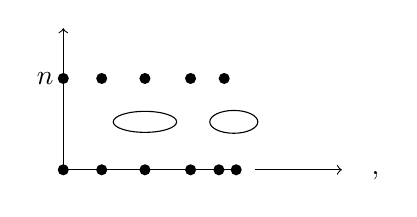
\begin{tikzpicture}[x=.61cm,y=.58cm]
\draw (0,0)--(3.6,0); \draw[->] (4.0,0)--(5.8,0);
\draw[->] (0,0)--(0,3.1);
\node[left] at (0,2.0) {$n$};
\foreach \x in {0,.8,1.7,2.65,3.24,3.6}{\fill (\x,0) circle (2pt);}
\foreach \x in {0,.8,1.7,2.65,3.35}{\fill (\x,2.0) circle (2pt);}
\draw (1.7,1.05) ellipse (.66 and .23); \draw (3.55,1.05) ellipse (.5 and .25);
\node at (6.5,-.12) {,};
\end{tikzpicture}}
% L7
donc on trouve la suite exacte
% L8–10
\[
\scriptstyle 0\to H^n(Y,F)\to H^n(X,\deleted{\unsure{f^*}}F_X)
\xrightarrow{\alpha}H^0(Y,\underbrace{H^n(Z,\overbrace{F_Z}^{\substack{M_Z\\\Vert}})}_{\substack{\Vert\\\mathrm{Hom}(\pi_n(Z,\unsure{z}),M)\\\text{par th. de Hurwicz}}})\longrightarrow H^{n+1}(Y,F)
\]
% L11–15
Ici \deleted{\unsure{$Z$}} je fixe un point $x$ de $X$, $Z$ désigne la fibre de $f$ en $y=f(x)$, et $M$ celle de $F$ en $y$, $M=F_y$. Le groupe $\pi_1(Y)$ y opère, d'ailleurs $\pi\overset{\mathrm{def}}{=}\pi_1(X,x)\unsure{\simeq|\xrightarrow{\sim}}\pi_1(Y,\unsure{y})$ aussi. Le $H^0(Y,H^n(Z,F_Z))$ peut s'interpréter, sauf erreur, comme
% L16
\[
\mathrm{Hom}_{\pi\deleted{\unsure{x}}}(\pi_n(Z;x),M),
\]
% L17–19
en tenant compte de l'opération de $\pi$ \inserted{$=\pi_1(X,x)$} sur $\pi_n(Z,\unsure{n|x})$ également. (À vérifier.) Il faut \unsure{interpréter} la flèche
% L20
\[
H^n(X,\deleted{\unsure{f^*}}F_X)\longrightarrow\mathrm{Hom}_{\pi}(\pi_n(Z,x),M),
\]
% L21
via l'application composée
% L22
\[
\pi_n(Z,z)\longrightarrow\pi_n(X,x)\longrightarrow H_n(X,\mathbb Z)
\tag*{(*)}
\]
% L23–24
Si $F$ est \uline{constant} sur $Y$ (p. ex. si $Y$ 1-connexe), donc de valeur $M$, on a les flèches can.
% L25–26
\[
\begin{aligned}
&\scriptstyle H^n(X,F_X)=H^n(X,M)\longrightarrow\mathrm{Hom}(H_n(X,\mathbb Z),M)\xrightarrow{\inserted{\text{grâce à la composition avec (*)}}}\mathrm{Hom}(\pi_n(Z,z),\\
&\hfill\scriptstyle M)
\end{aligned}
\tag*{($*'$)}
\]
% archive sheet number: 231
\scanpage{232}
\mspage{182}
% L1–2
et sûrement \deleted{(en dehors de toute hypothèse du type $b_n$ ou autre)} l'application canonique \inserted{\unsure{directe|dérivée|déduite} ``de localisation sur $Y$'', suivie de\ldots}
% L3
\[
H^n(X,F_X)\to H^0(Y,H^n(Z,F_Z))\to\mathrm{Hom}_\pi(\pi_n(Z),M)
\tag*{($\alpha$)}
\]
% L4–9
n'est autre que la \deleted{\unsure{$\simeq\mathrm{Hom}_{\pi}($}} composée des applications canoniques ci-dessus. Dans le cas actuel où on suppose $b_n$, la deuxième flèche dans ($\alpha$) est iso, donc la composée ``n'est autre'' que la flèche de localisation elle-même.
% L9–14
D'autre part $\pi_n(Z,z)\to\pi_n(X,x)$ dans ($*$) est nul, donc aussi $\pi_n(Z,\unsure{z|?})\to H_n(\unsure{X|Y},\mathbb Z)$, donc aussi la flèche composée ($*'$) qui s'en déduit. Revenant alors à la suite exacte de Leray (page précédente), on trouve que $H^n(\unsure{Y|X},F)\xrightarrow{\sim}H^n(X,\deleted{\unsure{f^*}}F_X)$.

% L15–19
\deleted{\unsure{Re}} Comment récupérer le cas où $F$ n'est \uline{pas} constant ? Dans le cas $n=2$, cela marchait, \deleted{\unsure{qui}} en passant \unsure{aux} rev. universels $\widetilde X,\widetilde Y$ de $X,Y$ \inserted{(pour pts $x,y$ choisis)}, et en écrivant les suites spectrales
% L20–21
\diagram{\begin{tikzcd}[ampersand replacement=\&,column sep=small]
H^*(Y,F)\arrow[d] \& E^{pq}_2\deleted{\unsure{\simeq}}\!=\deleted{\unsure{H}}H^p(\pi,H^q(\widetilde Y,F_{\widetilde Y})) \arrow[l,Rightarrow]\arrow[d]\\
H^{\unsure{*|n}}(X,F_X) \& E^{\prime pq}_2=H^p(\pi,H^q(\widetilde X,F_{\widetilde X})) \arrow[l,Rightarrow]
\end{tikzcd}}
% L22–24
L'hypothèse $b_n$ est conservée en passant de $f:X\to Y$ à $\widetilde f=\widetilde f_x:\widetilde X\unsure{-|\to}\widetilde Y$, donc on sait que
% archive sheet number: 232
\scanpage{233}
\mspage{183}
% L1
\[
E_2^{pq}\xrightarrow{\sim}E^{\prime pq}_2\qquad\text{iso si }q\leq n
\tag*{($\alpha$)}
\]
% L2
Dans le cas $n=2$, utilisant que
% L3
\[
E_2^{p1}=E^{\prime p1}_2=0\qquad\text{car }H^1(\widetilde X)=H^1(\widetilde Y)=0,
\]
% L4
on trouve deux suites exactes
% L3–4, right
\figure{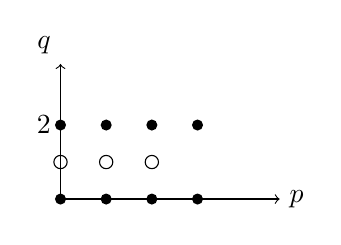
\begin{tikzpicture}[x=.58cm,y=.47cm]
\draw[->] (0,0)--(4.8,0) node[right] {$p$};
\draw[->] (0,0)--(0,3.65) node[above left] {$q$};
\node[left] at (0,2) {$2$};
\foreach \x in {0,1,2,3}{\fill (\x,0) circle (2pt); \fill (\x,2) circle (2pt);}
\foreach \x in {0,1,2}{\draw (\x,1) circle (2.4pt);}
\end{tikzpicture}}
% L5–7
\diagram{\begin{tikzcd}[ampersand replacement=\&,column sep=tiny,row sep=large]
\unsure{\cdot|0}\arrow[r] \& H^2(\pi,H^0(\widetilde Y))\arrow[r]\arrow[d,"\mathrm{iso}"] \& H^2(Y)\arrow[r]\arrow[d] \& H^0(\pi,H^2(\widetilde Y))\arrow[r]\arrow[d,"\mathrm{iso}"] \& H^3(\pi,H^0(\widetilde Y))\arrow[d,"\mathrm{iso}"]\\
0\arrow[r] \& H^2(\pi,H^0(\widetilde X))\arrow[r] \& H^2(X)\arrow[r] \& H^0(\pi,H^2(\widetilde X))\arrow[r] \& H^3(\pi,H^0(\widetilde Y))
\end{tikzcd},}
% L8–10
et un hom de l'une dans l'autre, qui permet de conclure par le lemme des 5 que $H^2(Y;F)\to H^2(X,F_{\unsure{x|X}})$ est iso.
% L10–16
Mais pour $n$ quelconque, la relation ($\alpha$) sur les termes $E_2$ \inserted{(pour $q\leq n$)} ne me semble pas impliquer la relation similaire pour les $E_r$ supérieurs, et de là pour les termes $E_\infty$, ce qui permettrait de conclure\unsure{.}

% L17–19
Je reviens donc à la suite exacte p. \unsure{187|181}, avec $F$ faisceau \uline{tordu}. J'ai envie de trouver une application canonique
% L20
\[
H^n(X,\unsure{G|E|\mathcal G})\longrightarrow\overbrace{\mathrm{Hom}_{\pi}(\pi_n(X,x),G_x)}^{\inserted{\substack{\text{Hom \uline{additifs} bien sûr}\\\text{i.e. en }\mathbb Z[\pi]\text{-modules}}}}, 
\]
% L21–22
où $G$ est un faisceau abélien loc. constant \unsure{quelc.} sur $X$, et $\pi=\pi_1(X,x)$. Si j'interprète
% archive sheet number: 233
\scanpage{234}
\mspage{184}
% L1–2
$\pi_n(X,x)$ par des classes d'homotopie d'applications ponctuées
% L3
\[
(S^n,x_0)\xrightarrow{\varphi}(X,x)
\]
% L4
j'ai bien, pour une telle application $\varphi$,
% L5
\[
\varphi^*:H^n(X,\unsure{G|C})\to H^n(S^n,\overbrace{\varphi^*\deleted{\unsure{(G)}}G_{\deleted{\unsure{x_0}}}}^{\simeq(G_x)_{S^n}})\simeq G_{\unsure{x|x_0}}
\]
% L6–9
(tenant compte que $S^n$ est 1-connexe, et que sa $n$-cohomologie à val. dans un faisceau constant $M$ est $M$. Sûrement l'application
% L10
\[
H^n(X,G)\unsure{-|\to}G_x
\]
% L11–12
ainsi définie ne dépend que de la classe d'homotopie ponctuée de $\varphi$, d'où
% L13
\[
\pi_n(X,x)\times H^n(X\unsure{,}G)\longrightarrow G_x,
\]
% L14–18
et il faut de plus prouver a) que c'est compatible avec les opérations de $\pi=\pi_1(X,x)$, et b) que c'est additif en $\pi_n(X,x)$, pour avoir l'application \unsure{souhaitée|cherchée}
% L19
\[
\deleted{\unsure{f}}H^n(X,G)\unsure{-|\to}\mathrm{Hom}_\pi(\pi_n(X,x),G_x).
\]
% L20–23
Si j'admets ceci, il n'y a qu'un pas pour admettre aussi que la flèche qui nous \unsure{retient|retiendra} \unsure{vraiment} (dans la suite exacte p. 181)
% archive sheet number: 234
\scanpage{235}
\mspage{185}
% L1–2
\[
H^n(X,F_{\unsure{X|x}})\unsure{-|\to}\mathrm{Hom}_\pi(\pi_n(Z,x),\underset{\substack{\Vert\\ F_y}}{M})
\]
% L3–4
n'est autre que la composée de la flèche précédente (page précédente) pour $\unsure{G|C}=F_X$, avec
% L5
\[
\mathrm{Hom}_\pi(\pi_n(X,x),M)\to\mathrm{Hom}_\pi(\pi_n(Z,x),M)
\]
% L6
déduite de
% L7
\[
\pi_n(Z,x)\unsure{-|\to}\pi_n(X,x).
\]
% L8–13
Or cette flèche est nulle, par l'hypothèse $b_n$. Donc la flèche $\alpha$ dans la suite exacte page 181 est nulle, donc $H^n(Y,F)\to H^n(X,F_X)$ est iso, qed (mais il y a pas mal de travail de vérifications à faire\ldots)

% L14–19
$c_n\Rightarrow a_{n-1}$. On peut procéder par récurrence sur $n$ (NB l'énoncé a un sens même pour $n=1$, où il est prouvé, et $\unsure{=}$ $c_1\Rightarrow b_1$, et $b_1\Rightarrow a_0$, \inserted{plus généralement $b_n\Rightarrow a_{n-1}$,} immédiat par suite exacte d'homotopie.)
% L20–23
Donc on sait déjà, en plus de l'hypothèse $c_n$, qu'on a $a_{n-2}$ i.e. $Z$ est $(n-\unsure{2|3})$-connexe. Il faut prouver qu'il est \inserted{$\unsure{=}$} $(n-1)$-connexe, i.e. $\pi_{n-1}(Z)=0$. Le cas $n=2$ demande
% archive sheet number: 235
\scanpage{236}
\mspage{186}
% L1–4, continuation at head
peut-être une attention particulière, car on
ne sait pas \unsure{$=$} encore que $Z$ est $1$-connexe.
Mais \deleted{\unsure{par}} on sait que $c_2$ implique $c_1$, qui équivaut
à $b_1$, \unsure{donc on a}
% L5–9, three successive maps
\[
 \pi_1(X,x)\longrightarrow\pi_1(Y,y)\qquad\text{iso,}
\]
donc
\[
 \pi_1(Z,x)\unsure{-|\to}\pi_1(X,x)\qquad\text{\uline{nul}}
\]
donc
\[
 \pi_2(Y,y)\unsure{-|\to}\pi_1(Z,x)\qquad\text{épi,}
\]
% L10–14, condition on the first homotopy group
ce qui implique tout au moins que
$\pi_1(Z,\unsure{x|z})$ est \uline{abélien}. \deleted{\unsure{Donc il}} Il faut le
voir comme un $\pi$-Module, et prouver
sa nullité comme tel (moyennant $c_2$).

% L15–19, general case and spectral sequence
Passons au cas général. On a pour $F$ loc
constant abélien sur $Y$
\[
 H^*(X,F_X)\Longleftarrow
 \underbrace{E_2^{pq}\unsure{=|\Leftarrow|\ne}H^p(Y,H^q(Z,F_Z))}
 _{\substack{=0\ \text{si }0<q<n-1\\\text{car }Z\text{ est }(n-2)\text{-connexe}.}}
\]
% L20, small diagram at right
\figure{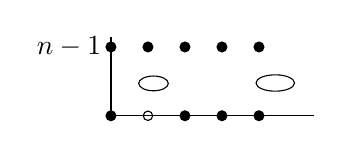
\begin{tikzpicture}[x=.47cm,y=.52cm]
 \draw (0,1.93)--(0,0)--(5.5,0);
 \node[left] at (0,1.68) {$n-1$};
 \foreach \x in {0,1,2,3,4} {\fill (\x,1.68) circle (2pt);}
 \foreach \x in {0,2,3,4} {\fill (\x,0) circle (2pt);}
 \draw (1,0) circle (1.7pt);
 \draw (1.15,.79) ellipse (.40 and .18);
 \draw (4.44,.80) ellipse (.52 and .20);
\end{tikzpicture}}
% L21–23, descending sequence at the foot
D'où
\[
 \begin{aligned}
 \scriptstyle 0\longrightarrow H^{\unsure{n-1|n}}(Y,F)\longrightarrow H^{n-1}(X,F_X)
 &\scriptstyle\longrightarrow\underbrace{H^0(Y,H^{n-1}(Z,F_Z))}
 _{\substack{\operatorname{Hom}_\pi(\pi_{n-1}(Z;x),F_x)\\\text{par Hurwicz}}}
 \\
 &\quad\searrow H^n(Y,F)\\
 &\qquad\qquad\searrow H^n(X,F_{\unsure{x|X}}\unsure{)}
 \end{aligned}
\]
% L24, unfinished at the lower edge
L'hypothèse $c_n$ implique qu'on a
% archive sheet number: 236
